\documentclass{standalone}
\usepackage{pgfplots}
\pgfplotsset{compat=1.15}
\usepackage{mathrsfs}
\usetikzlibrary{arrows, calc}
\newcommand{\degre}{\ensuremath{^\circ}}

\makeatletter
\def\convertto#1#2{\strip@pt\dimexpr #2*65536/\number\dimexpr 1#1}
\makeatother


\pagestyle{empty}
\begin{document}
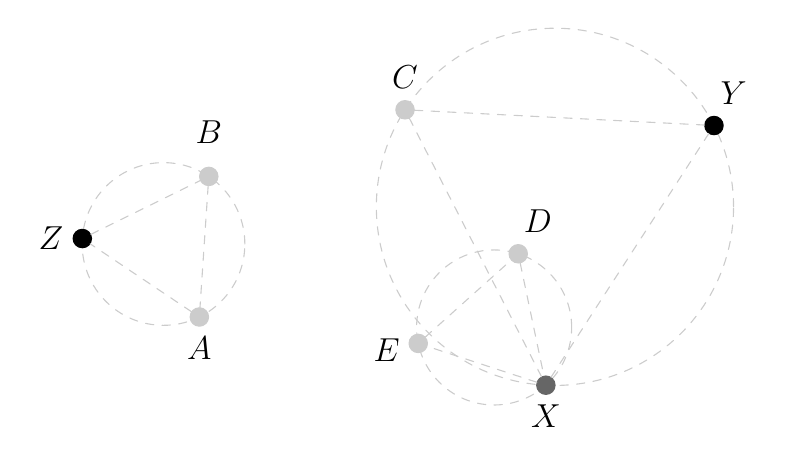
\begin{tikzpicture}[line cap=round,line join=round,x=9cm,y=9cm]
    % \clip (-0.8018777777777778, -0.06) rectangle (0.18692218302959018, 0.5178557671957673);    % E-D-X circumcircle
    % X-C-Y circumcircle
    \draw [dashed,gray!40] (-0.08843567026881602,0.26303977460768946) circle (0.2520269210900249);
    % % Z-A-B circumcircle
    \draw [dashed,gray!40] (-0.6408451590689551,0.2106249171823407) circle (0.1147882192237327);


    \begin{large}
        \draw [dashed,gray!40] (-0.1742873948409729,0.09281770574273644) circle (0.10941216875556445);

        \draw(-0.5902366791082465,0.10759522714775753) node[circle,draw=gray!40, fill=gray!40, scale=0.6] (A) [label={[yshift=-0.8cm]$A$}] {};
        \draw (-0.5769230701353238,0.30596799149252146) node[circle,draw=gray!40, fill=gray!40, scale=0.6] (B) [label={[yshift=0.15cm]$B$}] {};

        \draw (-0.3,0.4) node[circle,draw=gray!40, fill=gray!40, scale=0.6] (C) [label={$C$}] {};
        \draw (-0.14023669368546937,0.19679641713412993) node[circle,draw=gray!40, fill=gray!40, scale=0.6] (D) [label={[xshift=0.25cm]$D$}] {};
        \draw (-0.2813609509364418,0.07031712226437783) node[circle,draw=gray!40, fill=gray!40, scale=0.6] (E) [label={[xshift=-0.4cm, yshift=-0.5cm]$E$}] {};

        \draw (-0.10126453990100752,0.01133957782970145) node[circle,draw=black!60, fill=black!60, scale=0.6] (X) [label={[yshift=-0.8cm]$X$}] {};

        \draw (0.13595752909455952,0.3777797459933668) node[circle,draw=black,fill=black,scale=0.6] (Y) [label={[xshift=0.25cm]$Y$}] {};

        \draw (-0.7553757279632947,0.21831153290674304) node[circle,draw=black,fill=black,scale=0.6] (Z) [label={[xshift=-0.4cm, yshift=-0.4cm]$Z$}] {};
        \draw[dashed,gray!40] (E) -- (D) -- (X) -- (E) -- cycle;
        \draw[dashed,gray!40] (C) -- (Y) -- (X) -- (C) -- cycle;
        \draw[dashed,gray!40] (Z) -- (B) -- (A) -- (Z) -- cycle;



    \end{large}

\end{tikzpicture}
\end{document}